\section{Class \texorpdfstring{$\cls{M2}$}{M2}: the smaller-short window}\label{sec:smaller-short}

This section completes the exclusion of class $\cls{M2}$. By \cref{sec:mixed}, a competitive
normal period of class $\cls{M2}$ with at least six pieces has a global minimum of its active
margins at the centre of a reverse run (\cref{prop:m2-centre}). Of the two turns adjacent to that
centre we choose the one with the smaller active margin, and after reflecting and reversing time
if necessary (\cref{lem:m2-reflection}) it follows the centre. If the forward run that starts at
this turn has at least two switches, \cref{sec:mixed} excludes the period. The remaining case is a
forward run with a single switch: a short bridge between two reverse runs. Its data are fixed by
six real numbers, and no free continuation of the period is left to compare with. The proof
therefore works with a fixed list of necessary conditions on those numbers and shows that the list
is inconsistent.

The argument has seven steps, which we call gates, following the notes~\cite{Notes}
(\texttt{MIXED\_SMALLER\_SHORT\_HAND\_PERIOD\_EXCLUSION}). Gates S0 to S3 confine the shape of
the bridge to a small box, gate S4 gives a lower bound for the Casimir, gate S5 shows that the
bridge is sheared in a definite direction, and gate S6 shows that a bridge sheared in that
direction costs more, together with the rest of the period, than the octagon.

\subsection{The window}\label{sec:ss-window}

Index the pieces of the period so that piece $m$ is the global minimum. The seven pieces
$m-2,\dots,m+4$ have active margins
\[
  p_b,\; b,\; a,\; C,\; B,\; A,\; P_f,
\]
and the switches between them and after the last one have signs $+,-,-,+,-,-,+$. Thus $a$ is the
centre of a reverse run with the two turns $b$ and $C$; the turn $C$, the chosen smaller one, is
joined by the single forward switch $C\to B$ to the turn $B$; and $A$ is the centre of the next
reverse run, with far neighbour $P_f$. At a turn the two incident switch norms are equal
(\cref{lem:switch-norms}). Hence the three switches $a\to C$, $C\to B$, $B\to A$ of the bridge
share one norm, and we write $u$ for eight times it. Similarly $v$ is eight times the norm of the
switch $b\to a$ and $w$ eight times that of $A\to P_f$; the factor eight is the normalization of
the notes. The turn secant of \cref{lem:switch-norms} reads, in this normalization,
\begin{equation}\label{eq:ss-secant}
\begin{aligned}
  \operatorname{Sec}(A_0,B_0,P_0)&=1+\frac{B_0^2}{(A_0+B_0)(P_0+B_0)}
   -\frac{B_0}{P_0-A_0}\log\frac{P_0+B_0}{A_0+B_0}\\
   &=\frac{1}{P_0-A_0}\int_{A_0}^{P_0} g_{B_0}(s)\,\dd s,
\end{aligned}
\end{equation}
with $g_{B_0}(s)=1-B_0s/(B_0+s)^2$, and with the continuous value $g_{B_0}(A_0)$ at $A_0=P_0$.
The identity
\begin{equation}\label{eq:ss-g}
  g_{B_0}(s)=\frac34+\frac{(s-B_0)^2}{4(s+B_0)^2}
\end{equation}
shows that every secant lies in $[3/4,1]$. We also write $\mathcal U(s)=1-s+s^2$, so that
$g_{B_0}(A_0)=\mathcal U\bigl(A_0/(A_0+B_0)\bigr)$; this is four times the quantity $j_k$ of
\cref{lem:switch-norms}, and the switching inequalities of that lemma become $u\ge g$ at a forward
switch and $u\le g$ at a reverse one.

\begin{definition}[Smaller-short window]\label{def:ss-window}
A \emph{smaller-short window} consists of real numbers
$p_b,b,a,C,B,A,P_f$ (margins), $u,v,w$ (norms), $E,E_L$ (centre pairings) and $\Gamma$ (the
Casimir) such that, with $\rho=a^2/(a^2+4)$:
\begin{enumerate}[label=(\roman*)]
\item (order) $0<a<b$, $a<C\le b$, $a\le A<C$, $a\le p_b$, $A<B$ and $A<P_f$;
\item (strict star at the six switches) $p_bb$, $ab$, $aC$, $CB$, $BA$ and $AP_f$ are less
  than $4$;
\item (reverse centres) $(a+b)(a+C)<a^2+4$ and $(B+A)(A+P_f)<A^2+4$;
\item (scales) $2/15\le a$, $a^2<12/17$ and $A^2<12/17$;
\item (turn secants) $u=\operatorname{Sec}(a,C,B)=\operatorname{Sec}(C,B,A)$ and
  $v=\operatorname{Sec}(a,b,p_b)$;
\item (switching inequalities) $u\le g_C(a)$, $g_B(C)\le u$, $u\le g_B(A)$, $v\le g_b(a)$,
  $g_b(p_b)\le v$, $w\le g_{P_f}(A)$ and $3/4\le w$;
\item (centre stationarity) $E=\mathcal E(a,b,C,v,u)$ and $E_L=\mathcal E(A,B,P_f,u,w)$, where
  \[
    \mathcal E(a_0,p,n,u_i,u_o)=1+r'+t'-\rho_0+\log\frac{\rho_0}{r't'}-\frac{1-u_i}{r'}
    -\frac{1-u_o}{t'},
  \]
  with $r'=a_0/(a_0+p)$, $t'=a_0/(a_0+n)$ and $\rho_0=a_0^2/(a_0^2+4)$;
\item (Gram determinants and Casimir bounds)
  $\Gamma=(4uv-E^2)/(16(1-\rho)^2)$, $\Gamma=(4uw-E_L^2)/(16(1-\rho_A)^2)$ with
  $\rho_A=A^2/(A^2+4)$, and $27/256<\Gamma<9193/50000$;
\item (same-lift transport) $w=\lambda^2v+d^2u-d\lambda E$ and $E_L=2du-\lambda E$, where
  $\lambda=(a^2+4)/(A^2+4)$ and $d=\lambda\rho D$ with the bridge diagonal $D$ of
  \cref{tab:ss-variables};
\item (window defect) the inequality \eqref{eq:ss-defect} below, with $0<\mathcal B<\mathcal A$.
\end{enumerate}
\end{definition}

The conditions are the facts of \cref{sec:periods,sec:mixed} written at the seven pieces. The
orders come from the minimum structure (\cref{thm:class-M3}) and the choice of the smaller turn;
the products in (ii) and (iii) from the strict star condition and the reverse factors
(\cref{lem:one-arc}); the scales from the compact domain (\cref{thm:compact-domain}) and the
reverse-centre scale bound; and (v) to (ix) from
\cref{lem:stationarity,lem:switch-norms,lem:gram} applied to the one normal multiplier of the
period. The Casimir bounds are those of \cref{sec:mixed}.

\begin{table}[htbp]
\centering\small
\caption{The normalized variables of a smaller-short window. Lengths are divided by the central
margin $a$.}\label{tab:ss-variables}
\begin{tabular}{@{}ll@{}}
\toprule
Symbol & Definition \\
\midrule
$x,\ \beta,\ \alpha$ & $C/a$, $B/a$, $A/a$ (ratio, bridge, outer centre) \\
$\delta,\ \eta$ & $\beta/x-1=B/C-1$ (displacement); $(\alpha-1)/\delta$ \\
$\rho,\ r,\ t$ & $a^2/(a^2+4)$; $1/(1+x)=a/(a+C)$; $a/(a+b)$ \\
$q,\ r_A$ & $\rho_A=A^2/(A^2+4)$ (outer scale); $\alpha/(\alpha+\beta)=A/(A+B)$ \\
$q_c$ & $\alpha^2/(x(x+2)+\alpha^2)$, the value of $q$ at $\rho=r^2$ \\
$\tau,\ \tau_{\max}$ & $(A+P_f)/A$ (outer duration); $r_A/q$ \\
$\lambda,\ D$ & $(a^2+4)/(A^2+4)$; $\alpha^2+2\alpha\beta+1+2x-2\beta x$ (bridge diagonal) \\
$u,\ v,\ w$ & bridge, central and outer switch norms (times $8$) \\
$E,\ E_L$ & pairings at the centres $a$ and $A$ \\
$\Gamma,\ \kappa$ & the Casimir $\gamma^2$; $\sqrt{12\Gamma}$ \\
\bottomrule
\end{tabular}
\end{table}

\begin{proposition}[Extraction of the window]\label{prop:ss-extraction}
Let $P$ be a competitive normal period of class $\cls{M2}$ in the compact domain with at least six
pieces, let $m$ be a piece of least active margin, and suppose that the switches after pieces
$m-2,m-1,m,m+1,m+2$ have the signs $+,-,-,+,-$ and that $a_{m+1}\le a_{m-1}$. Then the active
margins $a_{m-2},\dots,a_{m+4}$ are the margins of a smaller-short window.
\end{proposition}

The essential new condition is the window defect. Let $\cost_{\mathrm{br}}$ be the cost of the two
bridge pieces, let $\theta_{\mathrm{br}}$ be the angle swept over the bridge by the continuous
polar angle of the costate frame, and let $\kappa=\sqrt{\det\Lambda_1}=\sqrt{12\Gamma}$. Over a
competitive period the polar angle increases by exactly $\pi/3$. The cost–Casimir inequality
(\cref{prop:cost-casimir}) has a pointwise strengthening: the cost density is at least
$\kappa+3/2$ times the rate of the polar angle (\texttt{GLOBAL\_SPECTRAL\_COST\_CASIMIR}
in~\cite{Notes}). Integrating it over the complement of the bridge gives
\begin{equation}\label{eq:ss-defect}
  \cost_{\mathrm{br}}+\Bigl(\kappa+\frac32\Bigr)\Bigl(\frac\pi3-\theta_{\mathrm{br}}\Bigr)
  \le\cost(T,X)\le\Aoct .
\end{equation}
Both sides are explicit.
Because the two turn secants agree, the logarithms in the two arc costs cancel and
\begin{equation}\label{eq:ss-cost}
  \cost_{\mathrm{br}}=\sqrt3\Bigl[\frac{\rho u}{1-\rho}(2\beta x-x-\alpha\beta)
   +\frac{\beta x-\alpha}{(1+x)(\alpha+\beta)}\Bigr],
\end{equation}
by the rational identity
$\frac{x(\beta-1)}{(1+x)(\beta+x)}+\frac{\beta(x-\alpha)}{(\alpha+\beta)(\beta+x)}
=\frac{\beta x-\alpha}{(1+x)(\alpha+\beta)}$. The angle is
$\theta_{\mathrm{br}}=\arctan(\sqrt3\mathcal B/\mathcal A)\in(0,\pi/3)$, where $\mathcal A$ and
$\sqrt3\mathcal B$ are $T_\kappa=2\kappa(1-\rho)^2$ times the real and imaginary parts of the product of the polar
coordinates of the costate frame at the two ends of the bridge. In the coordinates of
\cref{tab:ss-variables} they are rational functions of $x,\alpha,\beta,\rho,u,v,E$ and $\kappa$,
computed from the relative frame of the bridge and the costate at the central switch. The window
defect says that the bridge is cheap
compared with the angle it turns, and the gates show that no window satisfies it.

\begin{theorem}[The smaller-short window does not exist]\label{thm:m2-smaller-short}
There is no smaller-short window. Consequently no period
satisfies the hypotheses of \cref{prop:ss-extraction}.
\end{theorem}

The second sentence follows from the first by \cref{prop:ss-extraction}. It is the case of a short
forward run after the chosen smaller turn, and \cref{sec:mixed} uses it to finish class
$\cls{M2}$ (\cref{thm:class-M2}). The rest of this section proves the first sentence.

\subsection{Normalized data and the shape of the bridge}\label{sec:ss-normalized}

The secant is invariant under scaling of its three arguments, so in the variables of
\cref{tab:ss-variables}
\begin{equation}\label{eq:ss-equal-secants}
  u=\operatorname{Sec}(1,x,\beta)=\operatorname{Sec}(\alpha,\beta,x).
\end{equation}
The first secant averages $g_x$ over $[1,\beta]$ and the second averages $g_\beta$ over
$[\alpha,x]$. Only the conditions of \cref{def:ss-window} are used below. We collect the first
consequences.

\begin{lemma}[First consequences]\label{lem:ss-first}
Every smaller-short window satisfies:
\begin{enumerate}[label=(\alph*)]
\item $C\le B$, so that $1\le\alpha<x\le\beta$;
\item $u\le V(x):=\operatorname{Sec}(1,x,x)$, and $u\le13/16$;
\item $aB/C+\frac27(B-C)\le A$, that is $\alpha\ge\beta/x+\frac27(\beta-x)$, and in particular
  $\beta\le\alpha x$;
\item the outer centre is stationary: with $\tau=(A+P_f)/A$ one has $2<\tau<\tau_{\max}$ and
  \begin{equation}\label{eq:ss-root}
    E_L=(w-1)\tau+\frac1\tau+\frac{u-1}{r_A}+r_A+1-q+\log\frac{\tau q}{r_A};
  \end{equation}
\item $q\le q_c$ and $q<1/7$.
\end{enumerate}
\end{lemma}

\begin{proof}[Proof sketch]
(a) Suppose $B<C$. The cross inequality for secants gives
$\operatorname{Sec}(a,B,C)<\operatorname{Sec}(a,C,B)=u$. On the other hand, $g_B$ decreases on $[a,A]$ and
$g_B\ge g_B(A)\ge u$ there, so adding $[a,A]$ to the interval of $\operatorname{Sec}(A,B,C)=u$
gives $\operatorname{Sec}(a,B,C)\ge u$. (b) Split the integral of $\operatorname{Sec}(1,x,\beta)$
at $x$. On $[x,\beta]$ the integrand is at most $g_x(\beta)\le u$, the switching inequality at
$C\to B$, so $u\le V(x)$; and $V(x)\le13/16$ by a logarithm bound. (c) is the strengthened order
of the notes, proved by the comparison argument of \cref{app:ss-orders}. (d) is the
stationarity (vii) at $A$, rewritten: $\tau>2$ is $A<P_f$, and $\tau<\tau_{\max}$ is the reverse
factor at $A$. (e) $q\le q_c$ is equivalent to $\rho\le r^2$, which follows from $\rho<rt\le r^2$.
The bound $q<1/7$ is the reverse-centre scale bound of the notes, applied at the outer centre: if
$q\ge1/7$, the Gram determinant at $A$ would be at least $9193/50000$ (\cref{app:ss-scale}).
\end{proof}

Equation \eqref{eq:ss-root} is the one place where the outer reverse run enters. We write it as
$R_\tau(t,v)=0$, where the \emph{outer residual} $R_\tau(t,v)$ is the
right side of \eqref{eq:ss-root} minus $E_L$, with $w$ and $E_L$ given by the transport (ix) as
functions of the opposite turn $(t,v)$ and with $E$ given by the stationarity at $a$:
\begin{equation}\label{eq:ss-E}
  E(t,v)=(u-1)(1+x)+\frac{v-1}{t}+1+\frac{1}{1+x}+t-\rho+\log\frac{\rho(1+x)}{t}.
\end{equation}

The shape $(x,\alpha,\beta)$ is constrained by \eqref{eq:ss-equal-secants} alone. The gates use
it through explicit inequalities between $\alpha$ and $\beta$ at fixed $x$, which we call orders.

\begin{lemma}[Orders of the bridge]\label{lem:ss-orders}
Let $1<x$, $1\le\alpha<x\le\beta$ and $\operatorname{Sec}(1,x,\beta)=\operatorname{Sec}(\alpha,
\beta,x)$, and put $\delta=\beta/x-1$.
\begin{enumerate}[label=(\alph*)]
\item If $x\le9$, then $\alpha\ge\beta/x+k_s(x)(\beta-x)$ with $k_s(x)=4(x+1)/(7x+1)$.
\item $\alpha\le\beta/x+\frac54(\beta-x)$, and $\alpha\le\beta/x+\frac98(\beta-x)$ if $x\le5$.
\item If $x\le13/6$ and $\delta\le1/19$, then $\alpha\le1+3\delta$.
\item If $2\le x\le13/6$, then
  $\alpha\ge1+\frac{4x^2+11x+1}{7x+1}\,\delta+\frac{\delta^2}{1+4\delta}$.
\end{enumerate}
In particular, at a window with $x\ge2$ one has $\alpha\ge1+\bigl(1+\frac{4x(x+1)}{7x+1}\bigr)
\delta\ge1+\frac{13}{5}\delta$.
\end{lemma}

The last inequality holds because $4x(x+1)/(7x+1)$ increases, with derivative
$4(7x^2+2x+1)/(7x+1)^2$, and equals $8/5$ at $x=2$. In the slope $\eta=(\alpha-1)/\delta$, parts
(a) and (c) say that $\eta\in[13/5,3]$ on the box $2\le x\le13/6$, $0<\delta\le1/19$;
\cref{fig:smaller-short}(b) shows the actual slopes.

\subsection{How a gate compares the window with a face}\label{sec:ss-machinery}

Gates S0 to S4 share one structure. Each assumes that the window lies outside a region and
derives a scalar inequality at the actual window: $G\ge0$ for a weighted outer residual $G$, or
$\Gamma\ge G$ for a corrected Casimir $G$. It then moves the opposite turn, the scale and the outer
duration, each time in a direction that keeps the inequality valid, until the point reaches one of
two faces where all data are explicit functions of the shape $(x,\alpha,
\beta)$ and of $u$. There the inequality fails. We describe the moves once.

\runin{The opposite turn.} The norm $v$ and the ratio $t$ of the turn before the centre are not
controlled individually. They satisfy $v\le\mathcal U(t)$, the switching inequality at $b\to a$,
and $t_0:=\rho(1+x)\le t\le r$, from the central reverse factor and the choice of the smaller
turn. For a weight $m\ge0$ put $G=R_\tau+m(w-3/4)$. Then
\[
  \frac{\partial G}{\partial v}=\frac{\lambda}{t}B_{\tau+m}(t),\qquad
  \frac{\dd}{\dd t}G\bigl(t,\mathcal U(t)\bigr)=\frac{\lambda(2t-1)}{t}B_{\tau+m}(t),
\]
with the linear factor $B_z(s)=1+z(\lambda s-\lambda\rho D)$. When $B_{\tau+m}>0$ on $[t_0,t]$,
$G$ increases in $v$ and $G(s,\mathcal U(s))$ decreases in $s$ (since $s<1/2$), so
\begin{equation}\label{eq:ss-envelope}
  G(t,v)\le G\bigl(t_0,\mathcal U(t_0)\bigr)
\end{equation}. Without weight, the positivity of $B_\tau$ for
$\tau\le\tau_{\max}$ reduces to
$\alpha(\alpha+\beta)+(1+x)-D=x(\beta-1)+\beta(x-\alpha)>0$; with a weight each gate checks it separately. At the point
$(t_0,\mathcal U(t_0))$ the opposite turn has zero duration and the logarithm in \eqref{eq:ss-E}
vanishes.

\runin{The scale.} At $(t_0,\mathcal U(t_0))$ every quantity is rational in $\rho$. We
reparametrize by the outer scale $q=\rho_A$, through $\rho=q/(\alpha^2-(\alpha^2-1)q)$. Then
\begin{equation}\label{eq:ss-scale}
  w_*=1-qA_1+q^2A_2,\qquad E_{L,*}=-E_0+qA_3,\qquad
  E_0=(1+x)(u-1)+\frac{1}{1+x},
\end{equation}
with $A_1,A_2,A_3$ affine in $u$ and rational in $x,\alpha,\beta$. At fixed
$p=\tau q$ the residual becomes $R^*_{p/q}=\mathcal C(p)+q\mathcal L(p)$, where
$\mathcal C(p)=E_0+(u-1)/r_A+r_A+1-pA_1+\log(p/r_A)$ and $\mathcal L(p)=pA_2+1/p-1-A_3$. So at
fixed $p$ every weighted residual is a quadratic polynomial in $q$. The actual scale satisfies
$q\le q_c$ and $q<1/7$ (\cref{lem:ss-first}), and $q\le p/2$ because $\tau\ge2$.

\runin{The faces.} The scale is raised at fixed $p$ up to $q_{\max}=\min\{q_c,1/7,p/2\}$. If
$q_{\max}=p/2$, the duration has reached $\tau=2$, and the scale is raised further along $\tau=2$.
The end point lies on the \emph{central face} $q=q_c\le1/7$ or on the \emph{outer face}
$q=1/7\le q_c$. On the central face $\rho=r^2$, that is $(a+C)^2=a^2+4$: the central reverse
factor is one when both turns equal $C$, so the central piece has zero duration. On the outer face
the outer centre sits at the reverse-centre scale bound $A^2=2/3$. On each face all data are rational in $(x,\alpha,\beta,u)$,
except for the duration $\tau\in[2,\tau_{\max}]$ and the term $\log(\tau q/r_A)$.

\runin{The duration.} The duration enters only through $(w-1)\tau+1/\tau+\log\tau$. The identity
\begin{equation}\label{eq:ss-duration}
  R_\tau-R_2-(\tau-2)\Bigl(w-\frac34\Bigr)=\log\frac\tau2-\frac\tau4+\frac1\tau\le0
  \qquad(\tau\ge2)
\end{equation}
bounds every $R_\tau$ with $2\le\tau\le\tau_{\max}$ by $\max\{R_2,\,R_2+(\tau_{\max}-2)(w-3/4)\}$. A variant with two tangent lines to the logarithm reduces the duration to
three test values.

\runin{The incoming norm.} The bridge norm $u$ is the secant \eqref{eq:ss-equal-secants}, a
transcendental function of $(x,\beta)$. On each face the tested quantity is monotone in $u$, and
$u$ is replaced by a rational ceiling or floor, for instance
$V(x)\le\bar V(x)=\frac34+\frac{2(x-1)^2}{(x+1)(35x+13)}$ (\cref{app:ss-secant}). What remains is
the sign of an explicit function of $(x,\alpha,\beta)$, in some cases with one logarithm, on a
region bounded by the orders. These are the \emph{face signs}.

\subsection{Gates S0 to S3: the ratio and the displacement}\label{sec:ss-ratio}

The ratio $x=C/a$ is the shape parameter of the central reverse run, and the displacement $\delta$
measures how far the bridge is from symmetric. Gates S0 to S3 place $(x,\delta)$ in the box
$[2,13/6]\times[0,1/19]$ (\cref{fig:smaller-short}(a)).

\begin{figure}[htbp]
 \centering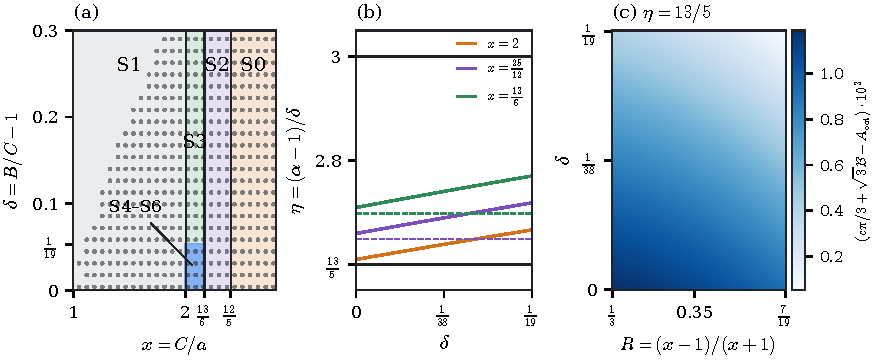
\includegraphics[width=\textwidth]{figures/fig-smaller-short.pdf}
 \caption{What the gates control. (a) The plane of the ratio $x=C/a$ and the displacement
 $\delta=B/C-1$. The dots are computed points of the equal-secant locus
 \eqref{eq:ss-equal-secants} with $1\le\alpha<x$. Gate S1 removes $x\le2$, S0 removes $x\ge12/5$,
 S2 removes $13/6\le x<12/5$ and S3 removes $\delta\ge1/19$, leaving the box where S4 to S6 work.
 (b) On that box, the slope $\eta=(\alpha-1)/\delta$ of the locus for $x=2,25/12,13/6$ (solid),
 between the lower order $1+4x(x+1)/(7x+1)$ (dashed) and the upper order $3$ of
 \cref{lem:ss-orders}. (c) The polynomial bound $\mathfrak B-b^*$ of gate S6 at $\eta=13/5$: it is
 positive on the whole box, with minimum $3.4\cdot10^{-5}$, small against
 $b^*=0.00223$.}\label{fig:smaller-short}
\end{figure}

\begin{proposition}[Gate S0]\label{prop:ss-S0}
Every smaller-short window has $x<12/5$, $D>0$ and $E_L>0$.
\end{proposition}

\begin{proof}[Proof sketch]
Suppose $x\ge12/5$. The root gives $R_\tau=0$ and $w\ge3/4$, so the floor-weighted residual
$G=R_\tau+\frac12(w-\frac34)$ is nonnegative at the actual window. Large ratios force a lopsided
outer bridge: the equal secants and $x\ge12/5$ give $\alpha/\beta<3/4$ and then
$D<\alpha(\alpha+\beta)$. The weighted envelope \eqref{eq:ss-envelope} applies (its factor stays
positive for $x>5/3$), so $G^*_\tau\ge0$ at the actual scale, and the two shape facts make
$G^*_\tau$ increase with $u$. At fixed $p$ its value at the zero scale is negative, and an endpoint argument
for the quadratic in $q$ gives a nonnegative value at $q_{\max}$; the move along $\tau=2$ keeps it
nonnegative. On the face reached, $u$ is raised to the ceiling $\hat u(x,\beta)$ (central face) or
$\bar u(x,\beta)$ (outer face), and the duration is reduced to the three tests $F(2,\cdot)$,
$F(8\tau_{\max}/9,\cdot)$, $F(\tau_{\max},\cdot)$ of \cref{sec:ss-machinery}. The three face
signs of \cref{prop:ss-face-S0} say that each test is negative on the region cut out by the
orders. This
contradiction gives $x<12/5$. For $x\le12/5$ the identities
\begin{align*}
  D-\bigl[(1+2x)\alpha^2-2x^2\alpha+1+2x\bigr]&=2(\beta-\alpha x)(\alpha-x),\\
  (1+2x)\alpha^2-2x^2\alpha+1+2x-D_0&=(\alpha-1)\bigl[(1+2x)(\alpha+1)-2x^2\bigr],
\end{align*}
with $D_0=2+4x-2x^2\ge2/25$, give $D\ge\alpha D_0>0$. Finally
$E_L=\lambda(2\rho Du-E)>0$, because $E$ is at most its envelope value
$(1+x)(u-1)+\frac1{1+x}+\rho(2x+1)$, which is less than $2\rho Du$.
\end{proof}

\begin{proposition}[Gate S1]\label{prop:ss-S1}
Every smaller-short window has $x>2$.
\end{proposition}

\begin{proof}[Proof sketch]
Suppose $1<x\le2$. For small ratios the residual alone is not enough, and the gate uses the upper
bound $\Gamma<9193/50000$. Moving the opposite turn changes the Casimir $\Gamma(t,v)$ computed at
the central reverse run, but the combination $\Gamma-\frac{7}{96}R_\tau$ does not increase along
the two moves of \eqref{eq:ss-envelope}: in $v$ it is concave with a nonpositive slope at the
actual point, and along $v=\mathcal U(s)$ its derivative is the derivative of $R_\tau$, which is
negative, times a factor that stays below zero. Since $R_\tau=0$ at the actual window,
\[
  \Gamma\ge\Gamma_*-\tfrac{7}{96}R^*_\tau
\]
at the actual scale, where $\Gamma_*$ is the Gram expression at
$(t_0,\mathcal U(t_0))$. At fixed $p$ the right side decreases in $q$, and along $\tau=2$ the slope
of $R^*_2$ in $q$ exceeds one, so the right side does not increase when the point moves to a face.
On the central face $q=q_c\le1/7$ and on the outer face $q=1/7\le q_c$, the face signs
$\Gamma_*-\frac{7}{96}R^*_\tau>9193/50000$ for every admissible duration
(\cref{prop:ss-face-S1}) contradict $\Gamma<9193/50000$.
\end{proof}

\begin{proposition}[Gate S2]\label{prop:ss-S2}
A smaller-short window with $x<12/5$ has $x<13/6$.
\end{proposition}

\begin{proof}[Proof sketch]
Suppose $13/6\le x<12/5$. The weight is now variable, $m=2-7\tau/(4\tau_{\max})\in[1/4,2)$, and
the weighted residual $G_\tau=R_\tau+m(w-3/4)$ is still nonnegative at the root. The envelope
applies with this weight, the scale polynomial is convex in $q$ with a negative value at the zero
scale, and the $\tau=2$ continuation reaches the face $q^*=\min\{q_c,1/7\}$. After raising $u$ to
the ceiling $u_C(x,\beta)$ on the central face, and to $u_s(x,\beta)$ or $\bar V(x)$ on the outer
face, the face signs $G_\tau<0$ of \cref{prop:ss-face-S2} give the contradiction.
\end{proof}

\begin{proposition}[Gate S3]\label{prop:ss-S3}
A smaller-short window with $2\le x\le13/6$ has $\delta<1/19$.
\end{proposition}

\begin{proof}[Proof sketch]
Suppose $\delta\ge1/19$. The displacement is penalized by the weight
$m=4(4-3\tau/\tau_{\max})/(5\alpha-1)$, with which $G_\tau=R_\tau+m(w-3/4)\ge0$ at the root. On
this range $\beta<2\alpha$, so $D=\alpha^2+1+2x+2\beta(\alpha-x)>5\alpha^2-4\alpha x+1+2x\ge
6-2x>0$. The same three moves reach the face $q^*=\min\{q_c,1/7\}$. The duration is reduced to two
tests, $F_0$ at $\tau=2$ and $F_1$ at $\tau=\tau_{\max}$, the norm is raised to a ceiling, and on
the central face a monotonicity in $\beta$ moves the point to the curve
$\beta=x+\frac{25x}{15x+36}(\alpha-1)$. The face signs $F_0,F_1<0$ of
\cref{prop:ss-face-S3} give the contradiction.
\end{proof}

\subsection{Gate S4: the small box and a floor for the Casimir}\label{sec:ss-S4}

After gates S0 to S3 the shape lies in $2<x<13/6$, $0\le\delta<1/19$. Gate S6 needs a two-sided
control of $\alpha$ in terms of $\delta$, and also a lower bound for $\kappa$, because the
completion term in \eqref{eq:ss-defect} is weighted by $\kappa+3/2$.

\begin{proposition}[Gate S4]\label{prop:ss-S4}
A smaller-short window with $2\le x\le13/6$ and $\delta\le1/19$ has $\alpha\le1+3\delta$ and
$\Gamma>1829/10000$.
\end{proposition}

\begin{proof}[Proof sketch]
The first inequality is \cref{lem:ss-orders}(c), proved by the comparison argument with a barrier
of slope $2/x$. For the second, the monotonicity used in gate S1, now with the constant $1/7$,
gives $\Gamma\ge\Gamma_*-R^*_\tau/7$ at the actual scale. The scale
is moved at fixed $p$, and along $\tau=2$, up to the central scale $q_c$, and the duration maximum
\eqref{eq:ss-duration} leaves the two functions
\[
  \Phi=\Gamma_*(q_c)-\tfrac17R^*_2(q_c),\qquad
  \Psi=\Phi-\tfrac17(\tau_{\max}-2)\bigl(w_*(q_c)-\tfrac34\bigr).
\]
Both decrease in $u$, so the norm may be raised to its ceiling $\bar u(x,\beta)$
(\cref{app:ss-secant}). The face sign $\min\{\Phi,\Psi\}>1829/10000$ on the closed box
$2\le x\le13/6$, $0\le\delta\le1/19$, $\frac{13}{5}\delta\le\alpha-1\le3\delta$
(\cref{prop:ss-face-S4}) concludes.
\end{proof}

With \cref{lem:ss-orders} the window now lies in the \emph{small-shape domain}
\begin{equation}\label{eq:ss-small}
  2\le x\le\tfrac{13}{6},\qquad 0\le\delta\le\tfrac1{19},\qquad
  1+\tfrac{13}{5}\delta\le\alpha\le1+3\delta,
\end{equation}
that is $\alpha=1+\eta\delta$ with $13/5\le\eta\le3$ when $\delta>0$, and $\alpha=1$ when
$\delta=0$. No division by $\delta$ is used, so the symmetric boundary $\delta=0$ is included.

\subsection{Gate S5: the root forces a negative shear}\label{sec:ss-S5}

The defect inequality compares the cost of the bridge with the angle it turns, and both are
governed by one number. Let $M$ be the relative frame of the bridge, from the central switch to
the far switch. After a fixed rotation that depends only on $x$, its lower row does not depend on
$\rho$, and $\det M=1$ then determines the upper row up to one real parameter $h$, the
\emph{shear}. Put $R_x=(x-1)/(x+1)$, $T_s=(\beta-\alpha)/(\beta+\alpha)$,
$\mathcal U_1=\mathcal U(r)=(3+R_x^2)/4$, $\mathcal U_2=\mathcal U(r_A)=(3+T_s^2)/4$ and the
anisotropy $\nu=\mathcal U_1/\mathcal U_2-1\ge0$. Then
\begin{equation}\label{eq:ss-shear}
  \sqrt3\,h=\frac{(\beta x-\alpha)\bigl((x+2)\alpha+(2x+1)\beta\bigr)}
  {(1+x)^2(\alpha^2+\alpha\beta+\beta^2)}
  -2\,\mathcal U_1\,(2\beta x-x-\alpha\beta)\,\frac{\rho}{1-\rho}
\end{equation}. This is a strictly decreasing function of the central scale $\rho$, and the
bridge cost \eqref{eq:ss-cost} is affine in it:
\begin{equation}\label{eq:ss-cost-shear}
  \cost_{\mathrm{br}}=H_0-J_0h,\qquad J_0=\frac{3u}{2\,\mathcal U_1},\qquad
  H_0=\frac{\sqrt3}{2}\Bigl[\Bigl(1+\frac{u}{\mathcal U_1}\Bigr)R_x
   +\Bigl(1+\frac{u}{\mathcal U_2}\Bigr)T_s\Bigr].
\end{equation}
A more negative shear makes the bridge more expensive. Gate S5 shows that the actual outer root is
compatible only with a negative shear.

\begin{proposition}[Gate S5]\label{prop:ss-S5}
A smaller-short window in the small-shape domain \eqref{eq:ss-small} has
$q>\frac{29}{30}q_c$, $\sqrt3hR_x+\frac{13}{3}\nu<0$, $h<0$ and $-hR_x>\frac52\nu$.
\end{proposition}

\begin{proof}[Proof sketch]
Suppose $q\le q_b:=\frac{29}{30}q_c$. With weight zero, \eqref{eq:ss-envelope} and
\eqref{eq:ss-scale} give $\mathcal R(u;p,q):=\mathcal C(p)+q\mathcal L(p)\ge0$ at $p=\tau q$,
and $2q\le p\le r_A$. The residual $\mathcal R$ is affine and increasing in $u$
(\cref{app:ss-S5}), and $u\le\bar V(x)\le u_5:=\frac{755}{996}+\frac{x-2}{100}$, so
$\mathcal R(u_5;p,q)\ge0$. But $\mathcal R(u_5;p,q)<0$ on the whole closed region
$0\le q\le q_b$, $2q\le p\le r_A$: it is affine
in $q$ at fixed $p$, negative on $q=0$ by the tangent bound $\log y\le y-1$, and negative on the
faces $q=q_b$ and $p=2q$ by two tangent lines to the logarithm and convexity in $\beta$. Hence
$q>q_b$. Since $\rho/(1-\rho)=q/(\alpha^2(1-q))$,
\[
  (1-q)\Bigl(\sqrt3hR_x+\frac{13}{3}\nu\Bigr)=F-Gq,
\]
where $F=2W/(3(1+x)^3k_A)$ and $G=2V/(3\alpha^2(1+x)^3k_A)$, with
$k_A=\alpha^2+\alpha\beta+\beta^2$ and polynomials $W,V>0$ given in \cref{app:ss-S5}. So
$\sqrt3hR_x+\frac{13}{3}\nu<0$ as soon as $q>F/G$, and $q_b>F/G$ is the polynomial inequality
$29V-30W\bigl(x(x+2)+\alpha^2\bigr)>0$ on the small-shape domain. The last
two conclusions follow because $R_x>0$, $\nu\ge0$ and $13/(3\sqrt3)>5/2$, that is, $676>675$.
\end{proof}

\subsection{Gate S6: the completion is too expensive}\label{sec:ss-S6}

\begin{proposition}[Gate S6]\label{prop:ss-S6}
For a smaller-short window in the small-shape domain with $\Gamma>1829/10000$, $h<0$ and
$-hR_x>\frac52\nu$,
\[
  \cost_{\mathrm{br}}+\Bigl(\kappa+\frac32\Bigr)\Bigl(\frac\pi3-\theta_{\mathrm{br}}\Bigr)>\Aoct
\].
\end{proposition}

The proof lowers the left side in four steps to an explicit function of the shape.

\runin{Step 1: lowering $\kappa$.} Since $12\cdot\frac{1829}{10000}-(\frac{40}{27})^2
=\frac{23}{1822500}>0$, the floor of gate S4 gives $\kappa>\kappa_0=40/27$. Since
$\theta_{\mathrm{br}}<\pi/3$, we may replace $\kappa+3/2$ by $c=\kappa_0+3/2=161/54$.

\runin{Step 2: the angle in terms of the shear.} Let $\psi=\arctan(R_x/\sqrt3)+\arctan(T_s/\sqrt3)$
be the angle of the fixed lower row of the rotated frame, let $K=\nu+2+2\kappa_0/J_0$, and
\[
  \delta(h)=2\arctan\frac{\sqrt{h^2+\nu^2}-h}{K+\sqrt{K^2-\nu^2}}.
\]
In the rotated basis, $\mathcal A+i\sqrt3\mathcal B$ is, up to a positive factor and the rotation
by $\psi$, a quadratic polynomial in one unknown entry of the costate at the central switch. The
condition that its values stay on one side of the line through the origin at angle $\psi+\delta$
is a discriminant inequality, which holds at $\delta=\delta(h)$. This gives
$\theta_{\mathrm{br}}\le\psi+\delta(h)$ for the actual shear. With
\eqref{eq:ss-cost-shear}, the left side of the proposition is at least
$H_0+c(\pi/3-\psi)+\tilde F(\delta(h))$, where $\tilde F(\delta)=-J_0\tilde h(\delta)-c\delta$ and
$\tilde h$ is the inverse of $h\mapsto\delta(h)$.

\runin{Step 3: continuation to the central scale.} The shear decreases in $\rho$, and $\rho<r^2$.
Let $h_c<h<0$ be the shear at the central scale $\rho=r^2$ and $\omega_c=\delta(h_c)$. On
$[\delta(h),\omega_c]$ the derivative of $\tilde F$ has the sign of a quadratic $Q_c(H^2)$ in
$H=-\tilde h$. The hypothesis $-hR_x>\frac52\nu$, together with $H\le-h_c<7R_x^2/6$, makes
$Q_c(H^2)<0$ along the whole continuation (the barrier lemma of the notes, applied pointwise). So
$\tilde F$ decreases, and the left side is at least the central score
\[
  \mathcal F_c=\cost_c+c\Bigl(\frac\pi3-\psi-\omega_c\Bigr),\qquad
  \cost_c=\sqrt3\Bigl[\frac{u(2\beta x-x-\alpha\beta)}{x(x+2)}+\frac{R_x+T_s}{2}\Bigr]
\]. Here $\cost_c$ is the bridge cost \eqref{eq:ss-cost} at the
central scale.

\runin{Step 4: a polynomial bound.} The Taylor bound $\arctan y\le y-y^3/3+y^5/5$ for $y\ge0$,
elementary bounds for $\omega_c$ and for the central shear, and the two-sided bound
$u_q(R_x,\delta)\le u\le\frac34+\frac{R_x^2}{12}$ give
\[
  \mathcal F_c>\frac{c\pi}{3}+\sqrt3\,\mathfrak B(u_q;R_x,T_s,\delta)-\frac1{800000}
\], with $\mathfrak B$ the explicit rational function of \cref{app:ss-S6}. It is
concave in $T_s$, and $T_s$ is monotone in $\eta$, so its minimum over $13/5\le\eta\le3$ is
attained at an endpoint. At both endpoints
$\mathfrak B>b^*=\frac{792669623}{356040000000}$ for $\frac13\le R_x\le\frac7{19}$ and
$0\le\delta\le\frac1{19}$ (\cref{prop:ss-face-S6}, \cref{fig:smaller-short}(c)). The constant
$b^*$ is defined by $\frac{989}{571}b^*=\frac{3126055}{10^6}-\frac{c}{3}\cdot
\frac{314159265}{10^8}+\frac{1}{800000}$, so $\pi>314159265/10^8$, $\sqrt3>989/571$ and
$\Aoct<3126055/10^6$ give
\[
  \mathcal F_c>\frac{c}{3}\cdot\frac{314159265}{10^8}+\frac{989}{571}b^*-\frac1{800000}
  =\frac{3126055}{10^6}>\Aoct.
\]


\subsection{Proof of \texorpdfstring{\cref{thm:m2-smaller-short}}{the theorem}}\label{sec:ss-assembly}

Let a smaller-short window be given. Gate S0 gives $x<12/5$, gate S1 gives $x>2$, and gate S2
then gives $x<13/6$. Gate S3 gives $\delta<1/19$, gate S4 gives $\alpha\le1+3\delta$ and
$\Gamma>1829/10000$, and \cref{lem:ss-orders} gives $\alpha\ge1+\frac{13}{5}\delta$. So the
window lies in the small-shape domain \eqref{eq:ss-small}. Gate S5 gives $h<0$ and
$-hR_x>\frac52\nu$, and gate S6 then contradicts the window defect \eqref{eq:ss-defect}. \qed
